\documentclass[12pt]{article}
\usepackage[utf8]{inputenc}
\usepackage{pgfplots}
\pgfplotsset{compat=1.18}
\author{Mahir Labib Dihan}

\title{My first LaTeX}

\begin{document}

\begin{center}
    \begin{tikzpicture}
        \pgfplotsset{width=10cm}
        \begin{axis}[xmin=-2, xmax=2, ymin=-2, ymax=2,
                axis lines=middle,
                xlabel=$x$,
                ylabel=$y$]
            \addplot[color=red, dashed, samples=50]{-1+x^2};
            \addplot[color=blue, dashed, samples=50, domain=-1:1]{+1-x^2};
        \end{axis}
    \end{tikzpicture}
\end{center}



\begin{center}
    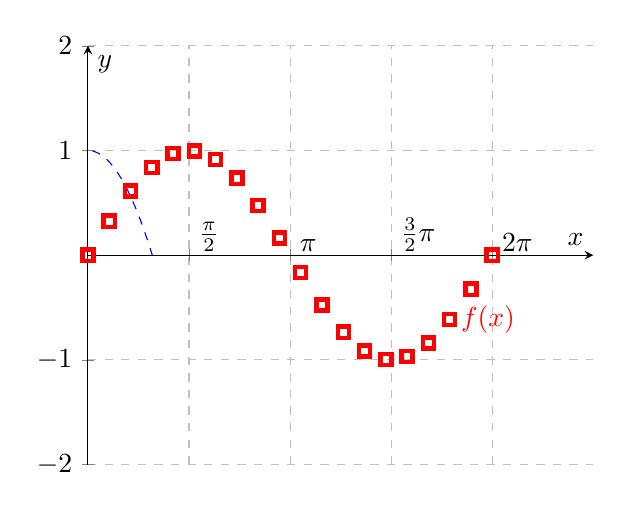
\begin{tikzpicture}
        \pgfplotsset{width=8cm}
        \begin{axis}[
                xmin=0, xmax=2.5*pi, ymin=-2, ymax=2,
                axis lines=middle,
                xlabel=$x$,
                ylabel=$y$,
                xmajorgrids=true,
                ymajorgrids=true,
                grid style=dashed,
                xtick={0,pi/2,pi,3*pi/2,2*pi},
                xticklabels={$0$,$\frac{\pi}{2}$,$\pi$,$\frac{3}{2}\pi$,$2\pi$},
                xticklabel style={anchor=south west}]
            \addplot[only marks,color=red,samples=20,mark=square,domain=0:2*pi,ultra thick]{sin(deg(x))}
            node[right,pos=0.9]{$f(x)$};
            \addplot[color=blue, dashed, samples=50, domain=-1:1]{+1-x^2};
        \end{axis}
    \end{tikzpicture}
\end{center}


\begin{center}
    \begin{tikzpicture}
        \pgfplotsset{width=15cm}
        \begin{axis}[scatter/classes={
                        a={mark=square}
                    }]
            \addplot[scatter, only marks, scatter src=explicit symbolic,mark size=5pt]
            coordinates{
                    (0.1,0.15)
                    (0.2,0.3)
                    (0.4,1.5)
                    (0.1,0.5)
                };
        \end{axis}
    \end{tikzpicture}
\end{center}

\begin{center}
    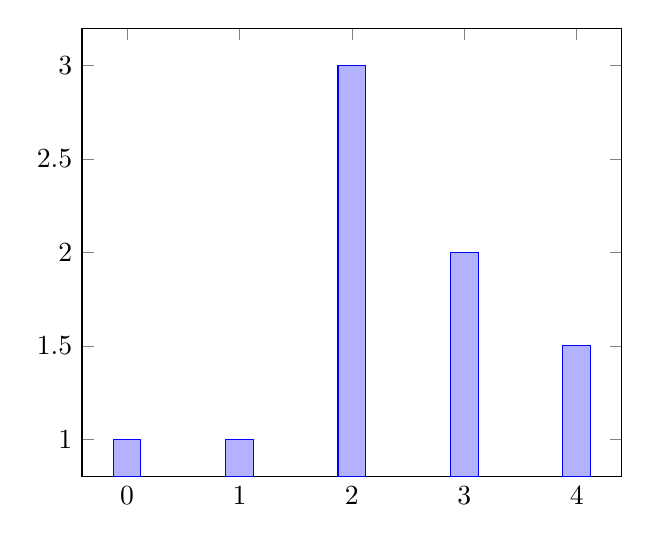
\begin{tikzpicture}
        \begin{axis}[ybar stacked]
            \addplot coordinates{
                    (0,1) (1,1) (2,3) (3,2) (4,1.5)
                };
        \end{axis}
    \end{tikzpicture}
\end{center}
\end{document}